\section{Graphical User Interface}
\label{sec:gui}
In order to ensure convenient and intuitive user interaction with the program, a graphical user interface (GUI) was implemented using the Qt5.4 \cite{Qt} framework. 
The GUI enables the user to enter all necessary files and parameters, eliminating any need for interaction through the command line. For supplying input files, the user needs to choose only the main \textit{.step} file. Assuming all other files were named according to the naming convention (see \autoref{sec: CADToVoxels}), activating the appropriate checkbox (for specifying fixtures or the optimization domain) should suffice. (see \autoref{fig:mainWindowParameters}).

All input parameters needed for topology optimization can be entered through text fields:
\begin{itemize}
\item Force Scaling - parameter for the scaling force magnitudes (see \autoref{sec: CADToVoxels}).
\item Resolution - parameter for calculating the voxel size for the voxelization. Voxel size is then equal to $2^{-(Resolution - 1)}$. Hence, by increasing the resolution the user reduces the length of the edge of a voxel by half, thus improving the accuracy of the solution.
\item Volume Fraction Limit - the fraction of the volume to be kept after the topology optimization process by ToPy (see sec. \ref{sec:ToPy}).

\end{itemize}
Similarly, all parameters necessary for surface fitting (see \autoref{sec:LSQfitting}) can be entered through text fields:
\begin{itemize}
\item Smoothing - parameter for the fairness functional (see \autoref{sec:NURBS})
\item Coarsening - the number of coarsening steps in Dual Contouring(see \autoref{ssec:parametrization}).
\end{itemize}

After all parameters have been specified, the pipeline can be executed without any intervention by the user. Progress of the program can be monitored by the dials present at the bottom of the GUI window. After completion of the process, the GUI provides an option to launch FreeCAD directly from the GUI and analyze the results.

\begin{figure}[h]
\centering
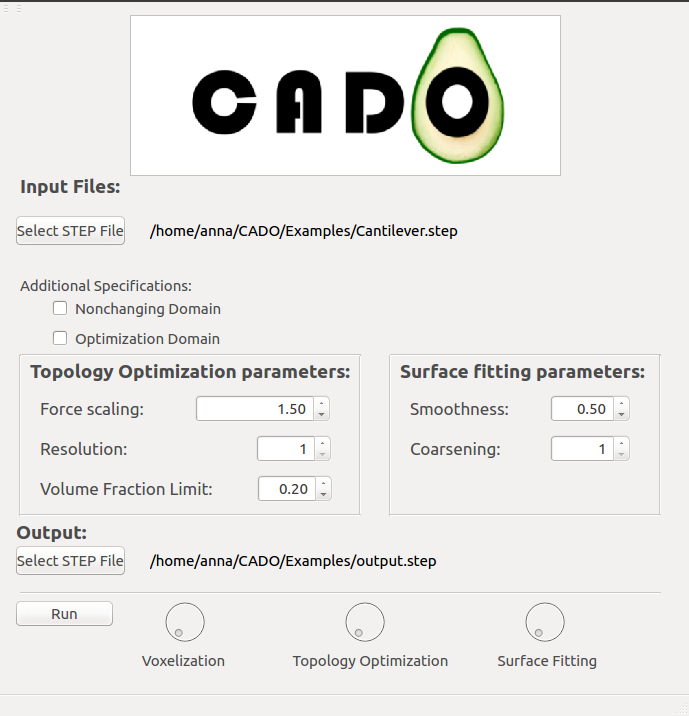
\includegraphics[scale=0.5]{Pictures/CADO_mainWindowParameters.png}
\caption{Program GUI showing file input and parameters for topology optimization and surface fitting. During execution of the program, the dials at the bottom indicate progress of the operation.}
\label{fig:mainWindowParameters}
\end{figure}